% -----------------------------------------------------------------
% Document class: Article
\documentclass[ a4paper, twoside, 11pt]{article}
\usepackage{../../../macros-general}
\usepackage{../../../macros-article}
% Number of the handout, quiz, exam, etc.
\newcommand{\numero}{02}
\setcounter{numero}{\numero}

% -----------------------------------------------------------------
\begin{document}
\allowdisplaybreaks

\begin{center}
\Large Mec\'anica Vectorial (MECG-1001): Lecci\'on \numero \\[2ex]
\small \textbf{Semestre:} 2017-2018 T\'ermino II \qquad
\textbf{Instructor:} Luis I. Reyes Castro \qquad
\textbf{Paralelo:} 09
\end{center}
\fullskip

% =============================================
\begin{problem} Dos varillas de 500 mm est\'an conectadas mediante un pasador en $D$ como lo indica la figura de abajo, donde todas las dimensiones se muestran en milimetros. El punto $B$ se mueve hacia la izquierda con una velocidad constante de 360 mm/s. 

\begin{figure}[htb]
\centering
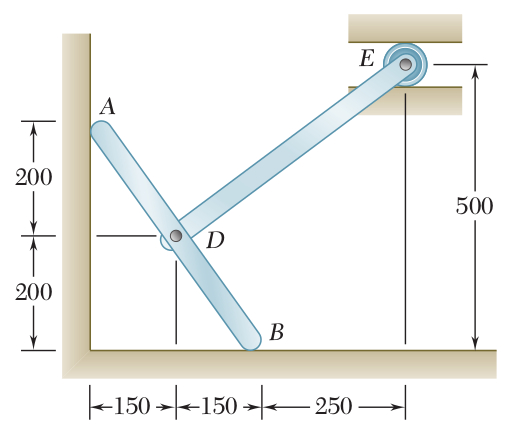
\includegraphics[width=0.46\textwidth]{problema-01.jpg}
\end{figure}

Complete las siguientes actividades: 
\begin{enumerate}[label=\textbf{\alph*)}]
\item \textbf{3 Puntos:} Encuentre la velocidad angular de la barra $AB$. 
\item \textbf{2 Puntos:} Encuentre la velocidad en $D$. 
\item \textbf{3 Puntos:} Encuentre la velocidad angular de la barra $DE$. 
\item \textbf{2 Puntos:} Encuentre la velocidad en $E$. 
\end{enumerate}

\end{problem}
\fullskip

% =============================================
\begin{problem}
Tres barras, cada una con un peso de 8 lb, est\'an soldadas entre si y se encuentran conectadas mediante pasadores a los dos eslabones $BE$ y $CF$, los cuales tienen peso despreciable y longitud de 10 in. 

\begin{figure}[htb]
\centering
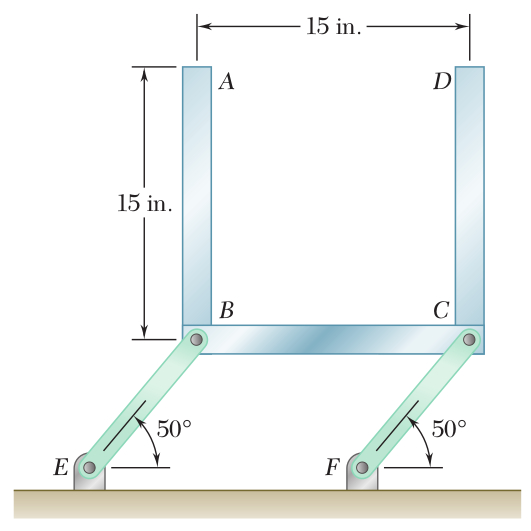
\includegraphics[width=0.46\textwidth]{problema-02.jpg}
\end{figure}

Complete las siguientes actividades: 
\begin{enumerate}[label=\textbf{\alph*)}]
\item \textbf{1 Punto:} Encuentre la locaci\'on del centro de masa del ensamble $ABCD$. 
\item \textbf{2 Puntos:} Encuentre la aceleraci\'on del centro de masa del ensamble $ABCD$ en funci\'on de la aceleraci\'on angular de la barra $BE$. 
\item \textbf{5 Puntos:} Determine la fuerza en cada eslab\'on inmediatamente despu\'es de que el sistema se suelta desde el reposo. 
\end{enumerate}

\end{problem}
\fullskip

% =============================================
\begin{problem}
\textbf{[6 Puntos]} Los extremos de una barra $AB$ de 9 lb est\'an restringidos a moverse a lo largo de ranuras cortadas en una placa vertical en la forma que se indica. Un resorte de constante $k = 3$ lb/in. se fija al extremo $A$ de manera tal que su tensi\'on es cero cuando $\theta = 0\deg$. La barra se suelta desde el reposo cuando $\theta = 50\deg$, determine la velocidad angular de la barra y la velocidad del extremo $B$ cuando $\theta = 0\deg$. 

\begin{figure}[htb]
\centering
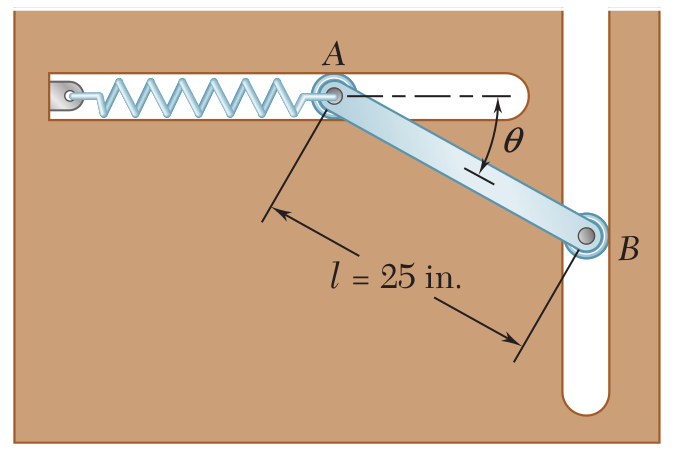
\includegraphics[width=0.5\textwidth]{problema-03.jpg}
\end{figure}

\end{problem}
\fullskip

\end{document}